% ============================================================
\chapter{L'Algorithme Mapper}
\label{ch:mapper}
% ============================================================

En 2007, Gurjeet Singh, Facundo M\'emoli et Gunnar Carlsson publient un article qui va transformer la TDA appliqu\'ee~: l'algorithme Mapper. L'id\'ee est d'une simplicit\'e remarquable~: au lieu de calculer l'homologie persistante d'un nuage de points (ce qui produit des invariants num\'eriques mais pas de visualisation directe), Mapper construit un \emph{graphe} qui capture la forme globale des donn\'ees. Le proc\'ed\'e s'inspire du th\'eor\`eme du nerf~: on d\'ecoupe les donn\'ees en morceaux chevauchants \`a l'aide d'une fonction filtre, on regroupe les points de chaque morceau par clustering, puis on relie les clusters qui partagent des points. Le graphe r\'esultant est une \og carte \fg{} des donn\'ees, d'o\`u le nom. Mapper a \'et\'e utilis\'e pour d\'ecouvrir un sous-groupe de cancer du sein, analyser la performance sportive, et explorer des donn\'ees g\'enomiques --- partout o\`u la visualisation de la \og forme \fg{} des donn\'ees apporte un \'eclairage inaccessible aux m\'ethodes statistiques classiques.

\begin{intuition}
Mapper est un algorithme de visualisation topologique qui construit un
graphe r\'esum\'e capturant la structure globale d'un jeu de donn\'ees
de haute dimension. Contrairement \`a l'homologie persistante qui
calcule des invariants num\'eriques, Mapper produit un objet
g\'eom\'etrique interpr\'etable.
\end{intuition}

% ============================================================
\section{Motivation}
% ============================================================

Les techniques de r\'eduction de dimension (PCA, t-SNE, UMAP) projettent
les donn\'ees dans un espace de faible dimension mais perdent
in\'evitablement de l'information structurelle. Mapper adopte une
approche diff\'erente~: il construit un graphe simplicial qui pr\'eserve
les propri\'et\'es topologiques du jeu de donn\'ees.

\begin{definition}[Reeb Graph --- Id\'ee sous-jacente]
Soit $f : X \to \R$ une fonction continue sur un espace topologique
$X$. Le \emph{graphe de Reeb} $\mathcal{R}_f(X)$ est le quotient de
$X$ par la relation~: $x \sim y$ si et seulement si $f(x) = f(y)$ et
$x, y$ sont dans la m\^eme composante connexe de $f^{-1}(f(x))$.
\end{definition}

Mapper est une \emph{approximation discr\`ete} du graphe de Reeb.

% ============================================================
\section{L'algorithme Mapper}
% ============================================================

\begin{algorithme}[title=\textbf{Algorithme Mapper (Singh, M\'emoli, Carlsson, 2007)}]
\textbf{Entr\'ees}~: Nuage de points $X$, fonction filtre
$f : X \to \R^k$, recouvrement $\mathcal{U}$ de $f(X)$,
algorithme de clustering $\mathcal{C}$.

\begin{enumerate}
  \item \textbf{Filtrage}~: appliquer $f$ pour obtenir
        $f(X) \subset \R^k$.
  \item \textbf{Recouvrement}~: choisir un recouvrement
        $\mathcal{U} = \{U_\alpha\}_{\alpha \in A}$ de $f(X)$ par des
        ouverts (typiquement des intervalles chevauchants).
  \item \textbf{Pr\'eimage et clustering}~: pour chaque $U_\alpha$,
        calculer $f^{-1}(U_\alpha) \cap X$ et appliquer l'algorithme
        de clustering $\mathcal{C}$, obtenant des clusters
        $C_{\alpha,1}, \ldots, C_{\alpha, k_\alpha}$.
  \item \textbf{Construction du nerf}~: construire le complexe
        simplicial dont les sommets sont les clusters et o\`u
        $\{C_{\alpha_0, i_0}, \ldots, C_{\alpha_p, i_p}\}$ forme un
        simplexe si et seulement si
        $C_{\alpha_0, i_0} \cap \cdots \cap C_{\alpha_p, i_p} \neq \emptyset$.
\end{enumerate}
\textbf{Sortie}~: le complexe simplicial (souvent un graphe, i.e., un
complexe de dimension~$1$).
\end{algorithme}

\begin{center}
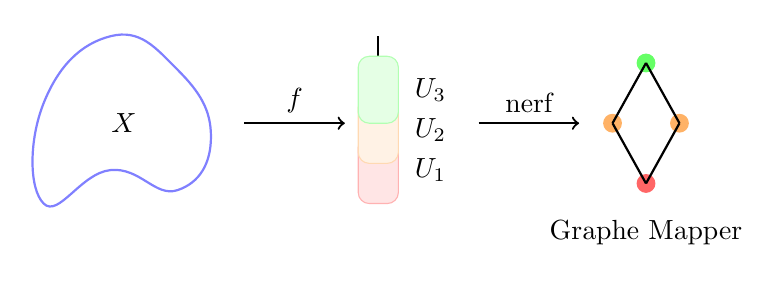
\begin{tikzpicture}[scale=0.85]
  % Data space
  \draw[thick, blue!50] plot[smooth cycle, tension=0.8]
    coordinates {(0,0) (1,0.5) (2,0.2) (2.5,1) (2,2) (1,2.5) (0,1.5)};
  \node at (1.2, 1.2) {$X$};
  \draw[->, thick] (3, 1.2) -- (4.5, 1.2) node[midway, above] {$f$};

  % Filter image
  \draw[thick] (5, 0) -- (5, 2.5);
  \draw[red!30, fill=red!10, rounded corners] (4.7, 0) rectangle (5.3, 1.0);
  \draw[orange!30, fill=orange!10, rounded corners] (4.7, 0.6)
    rectangle (5.3, 1.6);
  \draw[green!30, fill=green!10, rounded corners] (4.7, 1.2)
    rectangle (5.3, 2.2);
  \node[right] at (5.4, 0.5) {$U_1$};
  \node[right] at (5.4, 1.1) {$U_2$};
  \node[right] at (5.4, 1.7) {$U_3$};

  \draw[->, thick] (6.5, 1.2) -- (8, 1.2) node[midway, above] {nerf};

  % Mapper graph
  \fill[red!60] (9, 0.3) circle (4pt);
  \fill[orange!60] (8.5, 1.2) circle (4pt);
  \fill[orange!60] (9.5, 1.2) circle (4pt);
  \fill[green!60] (9, 2.1) circle (4pt);
  \draw[thick] (9, 0.3) -- (8.5, 1.2);
  \draw[thick] (9, 0.3) -- (9.5, 1.2);
  \draw[thick] (8.5, 1.2) -- (9, 2.1);
  \draw[thick] (9.5, 1.2) -- (9, 2.1);
  \node[below] at (9, -0.1) {Graphe Mapper};
\end{tikzpicture}
\end{center}

% ============================================================
\section{Choix des param\`etres}
% ============================================================

\subsection{Fonction filtre}

\begin{definition}[Fonctions filtres courantes]
\begin{itemize}
  \item \textbf{Coordonn\'ee}~: projection sur un axe, une composante
        principale.
  \item \textbf{Excentricit\'e}~: $f(x) = \left(\frac{1}{n}
        \sum_{i=1}^n d(x, x_i)^p\right)^{1/p}$.
  \item \textbf{Densit\'e}~: estimation par noyau (KDE),
        $k$-plus proches voisins.
  \item \textbf{Distance au $k$-\`eme voisin}~: mesure d'isolement.
  \item \textbf{Fonctions apprises}~: composantes de t-SNE, UMAP,
        autoencodeur.
\end{itemize}
\end{definition}

\subsection{Recouvrement}

\begin{definition}[Recouvrement par intervalles]
Pour une fonction filtre $f : X \to \R$, un recouvrement standard est
d\'efini par~:
\begin{itemize}
  \item $n_{\mathrm{int}}$~: nombre d'intervalles.
  \item $p_{\mathrm{ov}}$~: pourcentage de chevauchement ($0 < p_{\mathrm{ov}} < 1$).
\end{itemize}
La largeur de chaque intervalle est
$w = \frac{\max f - \min f}{n_{\mathrm{int}} - (n_{\mathrm{int}} - 1) p_{\mathrm{ov}}}$
et les intervalles sont~:
\[
  U_k = [\min f + k(1 - p_{\mathrm{ov}})w,\;
         \min f + k(1 - p_{\mathrm{ov}})w + w].
\]
\end{definition}

\begin{attention}[title=\textbf{Sensibilit\'e aux param\`etres}]
Le r\'esultat de Mapper d\'epend fortement du choix de la fonction
filtre, du nombre d'intervalles, du chevauchement et de l'algorithme de
clustering. Il est essentiel de faire varier ces param\`etres et
d'\'evaluer la robustesse du graphe r\'esultant.
\end{attention}

% ============================================================
\section{Impl\'ementation avec KeplerMapper}
% ============================================================

\begin{codeblock}[title=\textbf{Mapper avec KeplerMapper}]
\begin{minted}{python}
import numpy as np
import kmapper as km
from sklearn.datasets import make_circles
from sklearn.cluster import DBSCAN

# Données: deux cercles concentriques
X, y = make_circles(n_samples=500, noise=0.05, factor=0.5)

# Initialiser Mapper
mapper = km.KeplerMapper(verbose=1)

# Fonction filtre: projection sur la première coordonnée
lens = mapper.fit_transform(X, projection=[0])

# Construire le graphe Mapper
graph = mapper.map(
    lens, X,
    cover=km.Cover(n_cubes=15, perc_overlap=0.4),
    clusterer=DBSCAN(eps=0.3, min_samples=5)
)

# Visualisation HTML
mapper.visualize(
    graph,
    path_html="mapper_circles.html",
    title="Mapper: Cercles Concentriques",
    color_values=y
)
print(f"Nombre de noeuds: {len(graph['nodes'])}")
print(f"Nombre d'arêtes: {len(graph['links'])}")
\end{minted}
\end{codeblock}

% ============================================================
\section{Mapper avec GUDHI}
% ============================================================

\begin{codeblock}[title=\textbf{Mapper avec GUDHI}]
\begin{minted}{python}
import gudhi
import numpy as np

# GUDHI offre une implémentation de Mapper via
# la classe MapperComplex (versions récentes)

# Exemple conceptuel: construction manuelle
from sklearn.cluster import DBSCAN
from sklearn.neighbors import KernelDensity

X = np.random.randn(200, 3)

# Filtre: densité
kde = KernelDensity(bandwidth=0.5)
kde.fit(X)
f_values = kde.score_samples(X)

# Recouvrement
n_intervals = 10
overlap = 0.3
f_min, f_max = f_values.min(), f_values.max()
width = (f_max - f_min) / (n_intervals - (n_intervals - 1) * overlap)

clusters_all = []
for k in range(n_intervals):
    start = f_min + k * (1 - overlap) * width
    end = start + width
    mask = (f_values >= start) & (f_values <= end)
    if mask.sum() < 2:
        continue
    X_local = X[mask]
    db = DBSCAN(eps=0.5, min_samples=3).fit(X_local)
    labels = db.labels_
    for l in set(labels):
        if l == -1:
            continue
        idx = np.where(mask)[0][labels == l]
        clusters_all.append(set(idx.tolist()))

# Construire les arêtes (intersection non vide)
edges = []
for i in range(len(clusters_all)):
    for j in range(i+1, len(clusters_all)):
        if clusters_all[i] & clusters_all[j]:
            edges.append((i, j))

print(f"Noeuds: {len(clusters_all)}, Arêtes: {len(edges)}")
\end{minted}
\end{codeblock}

% ============================================================
\section{Fondements th\'eoriques}
% ============================================================

\begin{theoreme}[Convergence de Mapper --- Carri\`ere, Oudot, 2018]
Sous des conditions de r\'egularit\'e sur $f$ et $X$, lorsque le
nombre de points $n \to \infty$ et les param\`etres de recouvrement
sont choisis de mani\`ere adapt\'ee, le graphe Mapper converge (au sens
de la distance d'entrelacement fonctionnelle) vers le graphe de Reeb
de $(X, f)$.
\end{theoreme}

\begin{definition}[Distance d'entrelacement fonctionnelle]
Soient $\mathcal{R}_1$ et $\mathcal{R}_2$ deux graphes de Reeb. La
\emph{distance d'entrelacement fonctionnelle} est~:
\[
  d_{\mathrm{FI}}(\mathcal{R}_1, \mathcal{R}_2) =
  \inf_{\varepsilon} \{\varepsilon \geq 0 :
  \mathcal{R}_1 \text{ et } \mathcal{R}_2 \text{ sont }
  \varepsilon\text{-entrelac\'es}\}.
\]
\end{definition}

% ============================================================
\section{Mapper multidimensionnel}
% ============================================================

\begin{definition}[Mapper 2D]
Lorsque la fonction filtre est $f : X \to \R^2$, le recouvrement est
une grille de rectangles chevauchants dans $\R^2$. Le r\'esultat est un
complexe simplicial de dimension potentiellement $\geq 2$ (pas juste un
graphe).
\end{definition}

\begin{codeblock}[title=\textbf{Mapper 2D avec KeplerMapper}]
\begin{minted}{python}
import kmapper as km
import numpy as np
from sklearn.datasets import make_swiss_roll
from sklearn.cluster import DBSCAN

# Données: Swiss roll
X, color = make_swiss_roll(n_samples=1000, noise=0.5)

mapper = km.KeplerMapper()

# Filtre 2D: deux premières coordonnées
lens = mapper.fit_transform(X, projection=[0, 2])

graph = mapper.map(
    lens, X,
    cover=km.Cover(n_cubes=10, perc_overlap=0.3),
    clusterer=DBSCAN(eps=2.0, min_samples=5)
)

mapper.visualize(graph, path_html="mapper_swiss_roll.html",
                 color_values=color, title="Swiss Roll Mapper")
\end{minted}
\end{codeblock}

% ============================================================
\section{Applications c\'el\`ebres de Mapper}
% ============================================================

\subsection{Cancer du sein (Lum et al., 2013)}

L'\'etude fondatrice de Mapper en biologie a r\'ev\'el\'e des
sous-groupes dans les donn\'ees d'expression g\'enique du cancer du
sein qui n'avaient pas \'et\'e d\'etect\'es par les m\'ethodes de
clustering classiques.

\subsection{Analyse des joueurs de basketball (Lum et al., 2013)}

Mapper a \'et\'e appliqu\'e aux statistiques de joueurs de NBA,
r\'ev\'elant une structure en ``Y'' correspondant aux trois r\^oles
principaux (meneur, ailier, pivot).

\subsection{Diabète de type 2 (Li et al., 2015)}

Mapper a identifi\'e trois sous-types distincts de diab\`ete de type~2
\`a partir de donn\'ees cliniques, avec des implications th\'erapeutiques.

% ============================================================
\section{Coloration du graphe Mapper}
% ============================================================

\begin{remarque}
Le graphe Mapper est souvent color\'e par une variable d'int\'er\^et
(r\'eponse, label de classe, variable clinique) pour faciliter
l'interpr\'etation. Chaque n\oe{}ud re\c{c}oit la valeur moyenne de
la variable pour les points qu'il contient.
\end{remarque}

% ============================================================
\section{Ball Mapper}
% ============================================================

\begin{definition}[Ball Mapper --- D\l{}otko, 2019]
Le \emph{Ball Mapper} est une variante simplifi\'ee de Mapper o\`u~:
\begin{enumerate}
  \item On fixe un rayon $\varepsilon > 0$.
  \item On s\'electionne un sous-ensemble de points-rep\`eres
        $L \subset X$ (par farthest point sampling).
  \item Les n\oe{}uds sont les boules $B(l, \varepsilon)$ pour
        $l \in L$.
  \item Deux n\oe{}uds sont reli\'es si leurs boules contiennent des
        points communs.
\end{enumerate}
Avantage~: pas besoin de choisir une fonction filtre.
\end{definition}

% ============================================================
\section{Exercices}
% ============================================================

\begin{exercice}
Appliquer Mapper \`a un jeu de donn\'ees iris (\texttt{sklearn.datasets.load\_iris})
avec diff\'erentes fonctions filtres (PCA, excentricit\'e, densit\'e).
Comparer les graphes r\'esultants.
\end{exercice}

\begin{exercice}
\'Etudier l'effet du nombre d'intervalles et du pourcentage de
chevauchement sur le graphe Mapper. Pour un cercle bruit\'e, d\'eterminer
les param\`etres qui produisent un graphe cyclique.
\end{exercice}

\begin{exercice}
Impl\'ementer Ball Mapper en Python et l'appliquer \`a un nuage de
points en 3D.
\end{exercice}

\begin{exercice}
Montrer que si le recouvrement est suffisamment fin et l'algorithme de
clustering est exact, le graphe Mapper est une approximation du graphe
de Reeb de $(X, f)$.
\end{exercice}

\begin{exercice}
T\'el\'echarger un jeu de donn\'ees r\'eel (ex.~: donn\'ees g\'enomiques
d'expression) et appliquer Mapper pour identifier des sous-groupes.
Interpr\'eter le graphe r\'esultant.
\end{exercice}
